\documentclass{report}

\usepackage[spanish]{babel}
\usepackage[utf8x]{inputenc}
\usepackage{amsmath}
\usepackage{graphicx}
\usepackage[colorinlistoftodos]{todonotes}
\usepackage{enumitem}
\usepackage{listings}
\usepackage{verbatim}
\usepackage{eurosym}
\usepackage[export]{adjustbox}
\usepackage{amssymb}
\usepackage{bussproofs}
\usepackage{amsmath}
\usepackage{tikz}
\usepackage{xcolor}
\usepackage{listings}
\usepackage{titletoc}
\usepackage{hyperref}

\hypersetup{
  colorlinks=true,
  linkcolor=black,
  urlcolor=blue,
  citecolor=black
}

\newcommand{\coverPage}[6]{%
%----------------------------------------------------------------------------------------
%	COVER START
%----------------------------------------------------------------------------------------
\begin{titlepage}

    \newcommand{\HRule}{\rule{\linewidth}{0.5mm}}
    \newcommand{\department}{#1}
    \newcommand{\course}{#2}
    \newcommand{\titleValue}{#3}
    \newcommand{\subtitleValue}{#4}
    \newcommand{\authorName}{#5}

    \center

    %----------------------------------------------------------------------------------------
    %	HEADER
    %----------------------------------------------------------------------------------------
    
\includegraphics{images/logo_usa.png}
    \vspace{0.5cm}
    \textsc{\Large \department}\\[0.5cm]
    \textsc{\Large \course}\\[0.5cm]
    \vfill

    %----------------------------------------------------------------------------------------
    %	TITLE
    %----------------------------------------------------------------------------------------

    \HRule\\
    \Huge
    \textbf{\titleValue}\\[0.5cm]
    \Large
    \textbf{\subtitleValue}\\
    \HRule\\[0.5cm]

    %----------------------------------------------------------------------------------------
    %	AUTHOR AND DATE
    %----------------------------------------------------------------------------------------

    \vfill
    \Large
    \textit{\authorName}\\
    {\large \today}\\[2cm]

\end{titlepage}
%----------------------------------------------------------------------------------------
%	COVER END
%----------------------------------------------------------------------------------------
}

\begin{document}
    \coverPage{ Matemáticas }{ Geometría Euclidiana }{ Demostraciones congruencias de triángulos }{   }{ Alexander Mendoza }{\today}
    \tableofcontents
    \setlength{\parindent}{0pt}
    \pagebreak
    \chapter{ Demostraciones congruencias de triángulos }
    \section{Demostracion criterio de congruencia LLL}

    Dada la correspondencia entre el $\triangle ABC$ y $\triangle DEF$ tal que, $\overline{AB} \cong \overline{AC}$, $\overline{AC} \cong \overline{DF}$ y $\overline{BC} \cong \overline{EF}$, entonces, $\triangle ABC \cong \triangle DEF$.\\

    \textit{\textbf{Demostración}}. Para hacer la demostración haremos una construcción de la cual saldrán tres casos para demostrar. La construcción es la siguiente:\\

    Sean $\triangle ABC$ y $\triangle DEF$ tal que, $\overline{AB} \cong \overline{DE}$, $\overline{AC} \cong \overline{DF}$ y $\overline{BC} \cong \overline{EF}$, luego sea $G \in \mathcal{S}_{\overleftrightarrow{AC}, \neg B}$ de modo que $\angle CAG \cong \angle EDF$, así sea $H$ tal que $\overline{AG} \cong \overline{DE}$. Así $\triangle AHC \cong \triangle  DEF$, esto debido a congruencia LAL con $\overline{AH} \cong \overline{ED}, \angle HAC \cong \angle EDF$ y $\overline{DF} \cong \overline{AC}$. Luego $\overline{BH} \cap \overleftrightarrow{AC} = \{K\}$ esto por el PSP, intersección segmento puntos opuestos. Así tenemos tres casos para $K$.\\

    \textit{\textbf{Caso 1}}. Supongamos que $A - K - C$.
    \begin{center}
        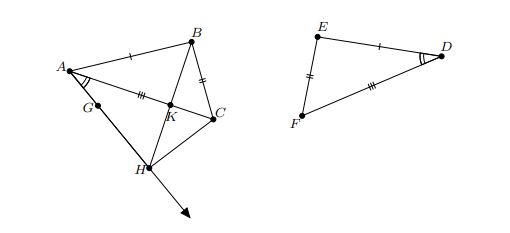
\includegraphics[height=4cm]{images/caso1.png}
    \end{center}

    Si $A - K - C$, entonces $\overline{AB} \cong \overline{AH}$ y $\overline{BC} \cong \overline{CH}$ esto por transitividad de congruencia. Así $\triangle ABH$ es isósceles, luego $\angle ABK \cong \angle AHK$, esto por definición de triángulo isósceles. De manera similar $\triangle BCH$ es isósceles y $\angle CBK \cong \angle CHK$. Luego $K \in int\angle ABC$ y $k \in int\angle AHC$ esto debido a la interestancia $A - K - C$ y el teorema interior de ángulo, lado opuesto de triángulo. Así $m\angle ABC = m\angle ABK + m\angle CBK$ y $m\angle AHC = m\angle AHK + m\angle CHK$. Por definición de congruencia de ángulos, $\angle ABC \cong \angle AHC$. Así $\triangle ABC \cong \triangle AHC$ por criterio de congruencia LAL. Por transitividad de congruencia $\triangle ABC \cong \triangle DEF$.\\

    \textit{\textbf{Caso 2}}. Supongamos que $A - C - K$.
    \begin{center}
        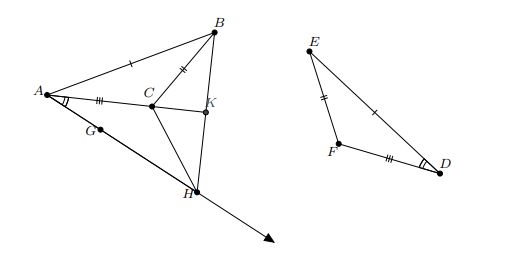
\includegraphics[height=4cm]{images/caso2.png}
    \end{center}

    Si $A - C - K$, entonces $\overline{AB} \cong \overline{AH}$ y $\overline{CB} \cong \overline{CH}$ esto por transitividad de congruencia. Luego el $\triangle ABH$ y el $\triangle CBH$ son isósceles, lo que implica que $\angle AHK \cong \angle ABK$ y $\angle CHK \cong \angle CBK$ esto debido a definición de triángulo isósceles. Debido a que $A - C - K$ sabemos que $C \in int\angle AHK$ y $C \in int\angle ABK$, por lo tanto $m\angle ABK = m\angle ABC + m\angle CBK$ y $m\angle AHK = m\angle AHC + m\angle CHK$, reemplazando ángulos congruentes tenemos que $m\angle AHC = m\angle ABC$. Luego por criterio de congruencia ALA tenemos que $\triangle AHC \cong \triangle ABC$. Así, por transitividad de congruencia, tenemos que $\triangle ABC \cong \triangle EDF$.\\


    \textit{\textbf{Caso 3}}. Supongamos que $K - A - C$.
    \begin{center}
        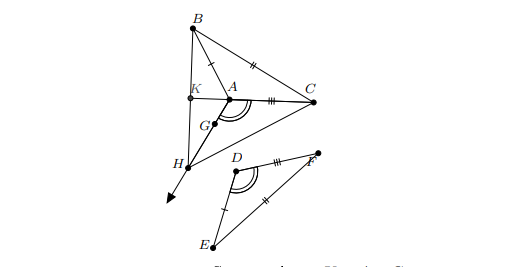
\includegraphics[height=5cm]{images/caso3.png}
    \end{center}

    De manera similar al anterior caso, si $K - A - C$, tenemos que $\angle CHA \cong \angle CBA$ lo que nos deja con un criterio de congruencia LAL con $\overline{AH} \cong \overline{BA}, \overline{CH} \cong \overline{CB}$ y $\angle CHA \cong \angle CBA$. Así $\triangle CAH \cong \triangle CAB$, y por transitividad de congruencia, $\triangle CAH \cong \triangle FDE$.\\

    De esta manera hemos demostrado que en cualquiera de los casos los triángulos son congruentes, por lo tanto el criterio de congruencia LLL se cumple.

    \section{Demostración del criterio de congruencia LAL usando como postulado ALA}

    Sean el $\triangle ABC$ y $\triangle FED$ tal que $\overline{BC} \cong \overline{ED}, \angle ACB \cong \angle FDE$ y $ \overline{AC} \cong \overline{FD}$ formando un criterio de congruencia LAL. Luego sea $G \in \mathcal{S}_{\overleftrightarrow{ED}, F}$ tal que $m\angle GED = m\angle ABC$, luego sea $F' \in \overleftrightarrow{DF} \cap \overrightarrow{EG}$, así $\angle F'ED \cong \angle ABC$. Por el postulado de criterio de congruencia ALA, $\triangle ABC \cong \triangle F'ED$. Esta congruencia implica que $\overline{F'D} \cong \overline{AC}$ y por transitividad de congruencia $\overline{F'D} \cong \overline{FD}$, lo cual implica que $F'D = FD$. Como $F' \in \overrightarrow{DF}$, esto ya que la totalidad de $\overrightarrow{EG}$ está en $\mathcal{S}_{\overleftrightarrow{ED}, F}$ y en particular $F'$ también lo está, entonces $F' = F$. Por lo tanto $\triangle ABC \cong \triangle FED$. Con esto demostramos la reciprocidad entre LAL y ALA.
\end{document}
